\documentclass[parskip=half,
 fontsize=12pt, bibtotoc,
 ngerman]
 {article}
%%Präambel
\usepackage[utf8]{inputenc} 
\usepackage[ngerman]{babel}
\usepackage{libertine}
\usepackage[T1]{fontenc}
%\usepackage{geometry}
\usepackage[bottom]{footmisc}
\usepackage{setspace}
\usepackage{anysize}
%Bibliographie
\usepackage{typearea}
\usepackage{biblatex}
\usepackage{amssymb}
\usepackage{amsmath}
\usepackage{algorithm}
\usepackage{algorithmic}
\usepackage{graphicx}
\renewcommand{\postnotedelim}{\addcolon\addspace}
%\usepackage[babel,german=guillemets]{csquotes}
\DeclareFieldFormat{postnote}{#1}
\bibliography{abschlussbericht}
\author{Terese Haimberger, Lea Helmers, Mahmoud Kassem, Daniel Theus, Moritz Walter}
\title{Abschlussbericht zum Softwareprojekt über Anwendungen effizienter Algorithmen -- WS 2013/14}
\date{}
\usepackage[left=3cm,right=4cm,top=2cm,bottom=2cm]{geometry}
\usepackage{hyperref}
\setlength{\parindent}{0pt}

\begin{document}

\thispagestyle{empty}
\maketitle
\begin{center}
\begin{Huge}
Rekonstruktion metrischer Graphen
\end{Huge}
\end{center}
\newpage
\thispagestyle{empty}
\tableofcontents
\newpage
\onehalfspacing
\section{Einleitung}
\subsection{Motivation und Problemstellung}
Im Rahmen des Softwareprojekts "`Anwendungen effizienter Algorithmen"' haben wir uns damit befasst, einen Algorithmus umzusetzen, der aus einer Punktmenge den zugrundeliegenden Graphen sowie dessen Metrik rekonstruiert. Dadurch soll Struktur in gro{\ss}e Mengen geometrischer Daten gebracht werden, was deren Analyse und Weiterverarbeitung erleichtert. Zu verarbeitende Daten können Netzwerke im weitesten Sinne sein, wie beispielsweise GPS-Daten, Strom- und Nachrichtennetze oder astrologische Daten. Häufig enthalten diese Daten Rauschen oder Ausreißer und sind zudem im Allgemeinen sehr umfangreich. Ziel des Algorithmus ist es, die Datenmenge kompakt durch ihre wichtigsten Verzweigungen darzustellen, wodurch sie auf ihre wichtigen Aspekte reduziert wird. So kann eine einfachere Visualisierung und die weitere Analyse und Verarbeitung der Daten ermöglicht werden.
\subsection{Der Algorithmus}
Als Grundlage für unsere Arbeit diente uns ein Paper \cite{chenEa2012}, welches einen Algorithmus für die Rekonstruktion metrischer Graphen beschreibt und dessen Richtigkeit beweist. Die Eingabe besteht dabei aus einem metrischen Raum $\left(Y, d_y\right)$, der aus den Rohdaten konstruiert wird und dem ein metrischer Graph $\left(X, d_x\right)$ zugrunde liegt, den es zu rekonstruieren gilt. Ziel des Algorithmus ist es, diesen zugrunde liegenden Graphen durch einen metrischen Graphen $(\hat{X}, d_{\hat{x}})$ anzunähern und dabei weitestgehend die Abstände von $\left(X, d_x\right)$ in $(\hat{X}, d_{\hat{x}})$ beizubehalten. Zusätzlich zu $\left(Y, d_y\right)$ wird auch ein Parameter $r$ übergeben, der in einigen Schritten des Algorithmus eine wichtige Rolle spielt. Die Erstellung des Graphen $(\hat{X}, d_{\hat{x}})$ wird nun wie folgt durchgeführt:\newline

\begin{enumerate}
\item \textbf{Kanten- und Knotenpunkte bestimmen}\newline
Zunächst wird festgestellt, welche der in $\left(Y, d_y\right)$ enthaltenen Punkte in $(\hat{X}, d_{\hat{x}})$ zu einer Kante und welche zu einem Knoten gehören werden. Dafür wird um alle im Eingabegraphen enthaltenen Punkte ein Kreisring gelegt, wobei der innere Kreis des Kreisrings den Radius $r$ und der äu"sere den Radius ${5\over 3}r$ hat. Für die Punktmenge in diesem Kreisring wird anschlie"send der Rips-Vietoris-Graph mit dem Parameter ${4 \over 3}r$ erstellt. Das bedeutet, dass alle Punkte, die nicht mehr als ${4 \over 3}r$ voneinander entfernt sind, zu einer Zusammenhangskomponente gefasst werden. Daraufhin wird der Grad des jeweiligen Knoten bestimmt, indem die Zusammenhangskomponenten des Rips-Vietoris-Graphen gezählt werden. Enthält der Kreisring um einen Knoten zwei Zusammenhangskomponenten, hat er Grad zwei und es handelt sich um einen Punkt, der im rekonstruierten Graphen $(\hat{X}, d_{\hat{x}})$ zu einer Kante gehören wird. Daher erhält er das Label \textit{edge point}. Ist der Grad ungleich zwei, wird der Punkt zu einem Knoten gehören und wird daher als \textit{preliminary branch point} gekennzeichnet.

\begin{figure}[h]
\centering
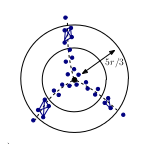
\includegraphics{branch.png}
\end{figure}

Diese Markierung erhalten diese Punkte lediglich vorläufig (\textit{preliminary}), da im Anschluss alle Punkte innerhalb eines Abstands von $2r$ von einem \textit{preliminary branch point} als \textit{branch point} gekennzeichnet werden. Hierbei werden auch die \textit{preliminary branch points} zu \textit{branch points}, womit sich die Punkte in $\left(Y, d_y\right)$ nun in zwei Teilmengen $\mathbb{E}$ und $\mathbb{V}$ aufteilen lassen. In $\mathbb{E}$ sind dabei die \textit{edge points} enthalten und in $\mathbb{V}$ die \textit{branch points}. Der Vorgang wird mit Pseudocode in Algorithm \ref{algo1} veranschaulicht. \newline
\begin{algorithm}
\caption{Kanten- und Knotenpunkte bestimmen}\label{algo1}
\begin{algorithmic}
\FORALL{$y \in Y$} 
\STATE $R \leftarrow C_{{5\over 3}r} \setminus C_r$ 
\STATE $deg\left(y\right) \leftarrow$ \# Zusammenhangskomponenten im Rips-Vietoris-Graphen$_{{4 \over 3}r}\left(R\right)$
	\IF{$deg(y) == 2$}
		\STATE y erhält das Label edge point
	\ELSE 
		\STATE y erhält das Label branch point
	\ENDIF
\ENDFOR
\FORALL{$y \in Y$}
	\IF{$y$ ist nicht weiter als $2r$ von einem preliminary branch point entfernt}
		\STATE y erhält das Label branch point
	\ENDIF
\ENDFOR
\end{algorithmic}
\end{algorithm}
\item \textbf{Struktur des Graphen rekonstruieren}\newline
Anschlie{\ss}end wird für die beiden Mengen $\mathbb{V}$ und $\mathbb{E}$ der Rips-Vietoris-Graph mit dem Parameter $2r$ erstellt. Die dabei entstehenden Zusammenhangskomponenten in $\mathbb{E}$ entsprechen nun den Kanten und jene in $\mathbb{V}$ den Knoten im Graphen $(\hat{X}, d_{\hat{x}})$. Um dessen Struktur zu vervollständigen müssen lediglich noch die Verbindungen zwischen Kanten und Knoten rekonstruiert werden. Dies geschieht, indem zwei Knoten aus  $\mathbb{V}$ genau dann durch eine Kante $e \in \mathbb{E}$ verbunden werden, wenn sie in ihrer Zusammenhangskomponente Punkte haben, die zu Punkten der Zusammenhangskomponente von $e$ einen kleineren Abstand als $2r$ haben.

\item \textbf{Metrik rekonstruieren}\newline
Schlussendlich müssen noch die Längen der Kanten bestimmt werden. Dafür wird jeder Kante in $\hat{X}$ als Länge der Durchmesser ihrer Zusammenhangskomponente, also der längste kürzeste Weg darin, zuzüglich $4r$ zugewiesen.
\end{enumerate} 


\section{Organisation}
\subsection{Programmiersprache}
Da allen Studenten im Team die objektorientierte Programmiersprache Java geläufig war und sie uns als durchaus geeignet für die Aufgabe schien, haben wir uns entschlossen, unser Programm darin zu schreiben.

\subsection{Gruppenaufteilung}
Für das Arbeiten an unserer Software haben wir uns in drei verschiedene Gruppen aufgeteilt. Die eine Gruppe hat sich mit der Vorverarbeitung der Rohdaten beschäftigt, im Wesentlichen also aus den Rohdaten den metrische Raum $\left(Y, d_y\right)$ für die Eingabe des Algorithmus konstruiert. Dabei beschlossen wir, uns auf die Visualisierung von GPS-Daten und Schwarz-Wei"sbildern zu beschr\"anken, sodass es vorrangig darum ging, diese beiden Datengrundlagen so aufzubereiten, dass die nächste Gruppe damit weiterarbeiten konnte. Die zweite Gruppe hat sich mit der Implementierung des Algorithmus, genauer der Rekonstruktion von $(\hat{X}, d_{\hat{x}})$, in Java auseinandergesetzt, während die dritte für die Visualisierung des Graphen $(\hat{X}, d_{\hat{x}})$ zuständig war.

\subsection{Kommunikation}
Damit wir stets alle über die Arbeit unserer Teammitglieder informiert waren, haben wir unsere Ergebnisse auf der Hosting-Plattform \textit{GitHub}\footnote{\url{github.com}} gespeichert und aktualisiert. Um anstehende Aufgaben für alle zugänglich zu dokumentieren haben wir zusätzlich die für Projektmanagement bestimmte Anwendung \textit{Trello} \footnote{\url{trello.com}} genutzt, bei der man ein virtuelles Notizbrett erstellen kann. Hier konnte jeder neue Aufgaben an eine virtuelle Pinnwand hängen und sich dafür als Bearbeiter eintragen. Zusätzlich konnten wir dort den Stand der Arbeit an diesen Aufgaben dokumentieren, wodurch stets jeder darüber informiert war, woran die anderen gerade arbeiteten.

Darüber hinaus haben wir per E-Mail kommuniziert und uns einmal pro Woche in der Universität getroffen, um die wichtigsten Ergebnisse der vergangenen und die Vorhaben für die kommende Woche zu besprechen und festzulegen.
 
\section{Arbeit in den einzelnen Gruppen}
Im Folgenden soll nun ein Überblick darüber gegeben werden, wie die drei verschiedenen Gruppen gearbeitet haben. Die Gruppe, die sich mit der Vorverarbeitung beschäftigt hat, bestand aus zwei Studierenden, jene, die für die Graphenrekonstruktion verantwortlich war, aus drei und für die Visualisierung des rekonstruierten Graphen war ein Student verantwortlich.

\subsection{Vorverarbeitung}
Die Kernaufgabe dieser Gruppe bestand in der Erfassung, sowie der Vorverarbeitung der Eingabedaten in eine für den Algorithmus passende Form.

Als Eingabe sind Schwarz-Weiß-Bilder, sowie GPS-Trace-Route-Dateien gedacht. Aus diesen müssen die Koordinaten der einzelnen Punkte extrahiert werden. Im Falle der GPS-Dateien wurde dazu ein Filter erstellt, welcher die angegebene Datei durchsucht und die Koordinaten (Längen- und Breitengrade) extrahiert. Sollte ein Bild angegeben werden, wird jeder Bildpunkt geprüft, wobei von jedem schwarzen die Pixelkoordinaten erfasst werden.

Da eventuell eine sehr große Punktmenge das Resultat sein kann, gibt es die Möglichkeit zur Reduzierung in Form der EpsilonNet-Klasse, welche durch Angabe eines Parameters (\emph{epsilon}) redundante Punkte entfernt. Dabei wird ein Algorithmus verwendet, der unter Verwendung eines Gitters ein metrisches Epsilon-Netz in linearer Zeit berechnet.\footnote{Sariel Har-Peled und Benjamin Raichel. Net and Prune: A Linear Time Algorithm for Euclidean Distance Problems. \url{http://web.engr.illinois.edu/~raichel2/aggregate.pdf}, 8. November 2012. (Der Algorithmus wird im Beweis zum Lemma 2.2 beschrieben.)}

Die Punkte werden in einem Set platziert und sind so zur weiteren Verarbeitung zugänglich.

Anschließend ist es das Ziel, diese Punkte in einen metrischen Raum (\textit{metric space}) umzuformen, d.\,h. die Punktmenge so zu strukturieren, dass wir möglichst schnell und einfach die paarweisen Abstände zwischen den Punkten berechnen können. Dazu wird zuerst die Delaunay-Triangulierung der Punktmenge berechnet (mithilfe der Delaunay\allowbreak TriangulationBuilder-Klasse der JTS Topology Suite). Anhand dieser Triangulierung wird ein Nachbarschaftsgraph erstellt. Der Graph besteht aus allen Knoten der Triangulierung und allen Kanten, deren Radius einen bestimmten Wert (\emph{alpha}) nicht überschreitet. (Der einzige Unterschied zum Alpha-Komplex ist, dass der Nachbarschaftsgraph keine Dreiecke enthält.) Als Datenstruktur werden dabei Adjazenzlisten verwendet.

Die Berechnung der Abstände erfolgt dann mithilfe des Floyd-Warshall-Algorithmus zur Bestimmung des kürzesten Pfades. Da diese Berechnung lange dauert, berechnen wir alle Abstände einmal und speichern sie in einer zweidimensionalen Tabelle (realisiert durch verschachtelte HashMap-Objekte). Bei der Rekonstruktion des Graphen können wir dann einfach auf die schon berechneten Abstände zugreifen.

Nun liegen alle benötigten Daten für den eigentlichen Algorithmus vor und werden in Form eines MetricSpace-Objektes übergeben.

\begin{figure}[h]
\centering
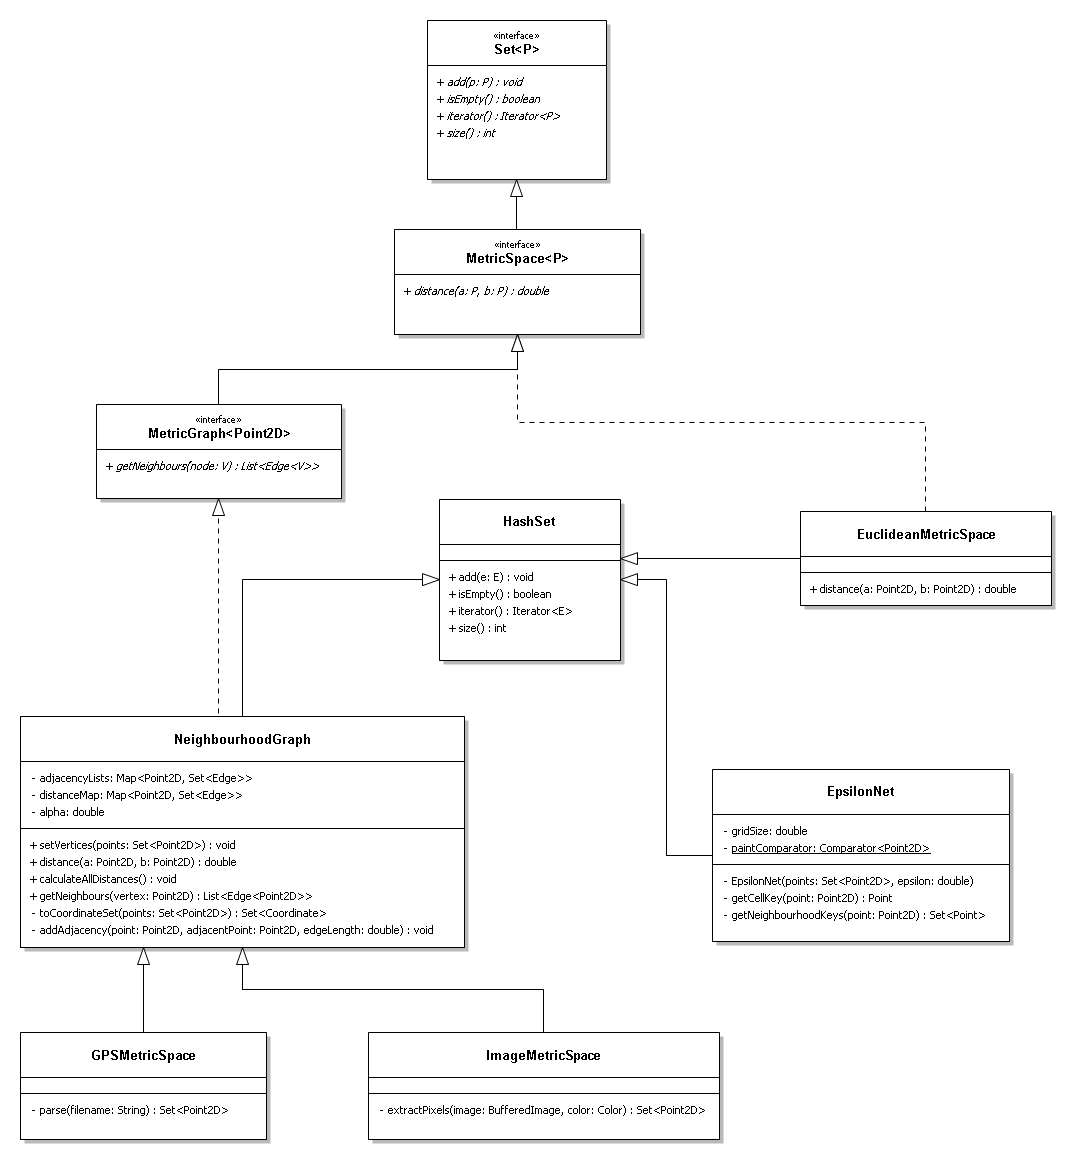
\includegraphics[scale=0.5]{preprocessing.png}
\caption{Klassendiagramm der Vorverarbeitung}
\end{figure}

\subsection{Rekonstruktion}

\begin{figure}[h]
\centering
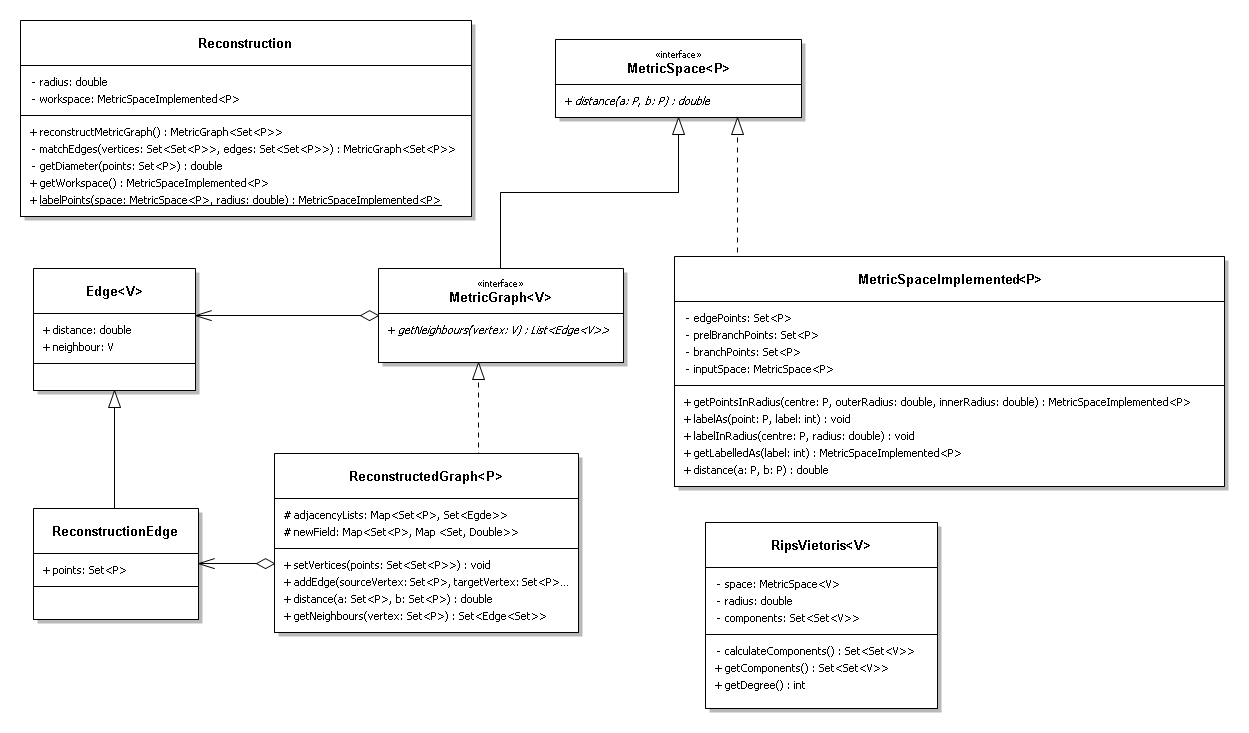
\includegraphics[scale=0.5]{main.png}
\caption{Klassendiagramm der Rekonstruktion}
\end{figure}

Die Aufgabe der Rekonstruktion ist es, mithilfe des Algorithmus und der aus der Vorverarbeitung gelieferten Daten den gesuchten Graphen aus der Punktmenge zu rekonstruieren. Dazu haben wir den Algorithmus selbst in der Klasse Reconstruction implementiert. Der Algorithmus benötigte jedoch ebenfalls den Rips-Vietoris-Graphen über bestimmte Punktmengen. Dieser wurde in der Klasse RipsVietoris implementiert. Da die Daten der Vorverarbeitung nur die Punkte sowie eine Distanzfunktion über diese Punkte gemäß der Schnittstelle MetricSpace umfasste, war es notwendig diesen MetricSpace zu erweitern, was durch die Klasse MetricSpaceImplemented geschieht. Dadurch dass die Rekonstruktionsgruppe aus 3 Mitgliedern bestand, hat jeder die Programmierung einer der Klassen übernommen. Die Aufteilung war wie folgt:

\begin{enumerate}
\item MetricSpaceImplemented: Lea Helmers
\item Reconstruction: Moritz Walter
\item RipsVietoris: Mahmoud Kassem
\end{enumerate}

Da die drei Klassen eng zusammenarbeiten, fand meist ein reger Austausch über ihren Aufbau in den Gruppentreffen und via E-Mail statt. Getestet wurden die Klassen später zunächst soweit möglich einzeln und dann als Modul. Dabei wurden unter anderem auch Testeingaben und eine vorläufige Anzeige für metrische Räume entwickelt. Als Endergebnis dieses Moduls gibt es den fertig rekonstruierten Graphen, abrufbar durch reconstructMetricGraph(), welcher dann durch die Visualisierung angezeigt werden kann.

\subsection{Visualisierung}

Die Visualisierung dient drei Zwecken:

\begin{enumerate}
\item \textbf{Testen:} Sie erlaubt es uns auf einen Blick zu sehen, ob unsere Implementierung das liefert, was wir erwarten.
\item \textbf{Parameterauswahl:} Sie ermöglicht es dem Benutzer, unterschiedliche Parameter auszuprobieren und zu sehen, wie sich dadurch die Zwischen- und Endergebnisse ändern.
\item \textbf{Vergleich der Ein- und Ausgabe:} Am Ende sieht der Benutzer eine graphische Darstellung des metrischen Raumes, zusammen mit dem rekonstruierten metrischen Graphen.
\end{enumerate}

Die graphische Benutzeroberfläche zur Visualisierung haben wir in zwei Fenster aufgeteilt: das Vorverarbeitungsfenster dient zum Testen der Vorverarbeitung und zur Auswahl der Parameter \emph{epsilon} und \emph{alpha}, während das Rekonstruktionsfenster zum Testen unserer Implementierung des Algorithmus, zur Auswahl des Parameters \emph{radius} und zum Vergleich der Ein- und Ausgabe dient.

Damit der Benutzer bei der Parameterauswahl nicht nach jeder Änderung der Parameter lange warten muss, bis er die Auswirkungen sieht, haben wir Vorschau-Schaltflächen eingebaut. Im Vorverarbeitungsfenster wird bei der Vorschau ein Nachbarschaftsgraph ohne Abstände berechnet. Wichtig bei der Auswahl von \emph{epsilon} und \emph{alpha} sind nämlich nicht die Abstände zwischen den Knoten, sondern die Struktur des Graphen. Im Rekonstruktionsfenster werden bei der Vorschau nur die Kanten- und Knotenpunkte bestimmt (die Kantenpunkte werden blau und die Knotenpunkte rot markiert).

Zur Benutzerfreundlichkeit gibt es in beiden Fenstern eine Statusanzeige. Falls eine Berechnung lange dauert, kann der Benutzer dort den Fortschritt verfolgen. An dieser Stelle werden auch die Kantenlängen bzw. die Koordinaten angezeigt, wenn der Benutzer mit der Maus über Kanten oder Knoten des rekonstruierten metrischen Graphen fährt.

\section{Testen}

Das Testen erwies sich anfangs als schwierig, denn benötigte Daten für ein Modul kamen meist aus einem anderen Modul und es war nicht auszuschließen, dass diese Daten bereits Fehler enthielten. Des Weiteren wurde anfangs das Ergebnis eines Moduls direkt an das nächste weitergeleitet ohne eine zwischenzeitliche Veranschaulichung, so dass die Daten auf Fehler gesichtet werden mussten. Aus diesem Grund entwickelten wir in den einzelnen Gruppen Hilfsprogramme zur Visualisierung des entsprechenden Zwischenergebnisses sowie einige Sets von festen Test-Eingabedaten. Es war jedoch etwas zweischneidig, da diese Visualisierungsprogramme zu Anfang ebenfalls Fehler enthielten, so dass zum Beispiel bei der Anzeige des Ergebnisses der Graph an verschiedenen Achsen gespiegelt wurde. Nach dem Beheben dieser Schwierigkeiten war es möglich, die meisten Funktionen erstmals rudimentär zu testen, bis dann schließlich ein Gruppenmitglied das komplette Modul im Zusammenspiel nochmals getestet hat.

Nachdem dies geschehen war, führten wir die Module zu einem Gesamtprogramm zusammen. Dabei sind unter anderem die Teilvisualisierungen mit in die Endvisualisierung eingeflossen. Nun wurde nochmals das komplette Programm als solches getestet, wobei hier kaum noch Schwierigkeiten auftraten, da die meisten Fehler durch die vorhergehenden Tests beseitigt wurden.

\section{Schwierigkeiten und Verbesserungsvorschläge}

\subsection*{Umsetzung des Algorithmus}
Eine grundsätzliche Schwierigkeit war das Testen fertiger Module.
Aufgrund der Datenfluss-artigen Struktur des Gesamtprogramms kann
ein kleiner Fehler in der Vorverarbeitung massiven Einfluss
auf das Endergebnis nehmen. Da dieses Ergebnis graphischer Natur ist,
war wirkliches Testen aber erst nach Erstellung einer graphischen Ausgabe
(Prototyp) möglich. Im Falle des Epsilon-Netzes ließ sich so beispielsweise 
zuverlässiges Aussortieren von nicht benötigten Punkten erst spät testen,
da sich anhand der blanken Koordinaten die Auswirkungen nicht gut genug
erkennen ließen und die Menge als Ganzes nur schwer zu erfassen war.

Ideen für weitere Features bzw. Änderungen an Algorithmen gab es einige. So waren
als Verbesserungen z.\,B. eine Einbeziehung des Zeitstempels von GPS Daten
zur Verbesserung des Nachbarschaftsgraphen, die Abstandsberechnung mithilfe des
Algorithmus von Dijkstra statt Floyd-Warshall um die Laufzeit zu senken,
eine automatisierte Möglichkeit zur optimalen Bestimmung der Parameter oder
auch die Berechnung von Orthodromen um den Abstand in km anzugeben, angedacht. Allerdings machte der Zeitmangel die Umsetzung zunichte.

\subsection*{Organisation}
Die zu erledigenden Aufgaben wurden von allen Gruppenmitgliedern stets sehr ernst genommen und möglichst schnell erledigt. Diese Zuverlässigkeit war grundlegend dafür, dass wir den Algorithmus letztendlich erfolgreich implementieren konnten. Bedauerlicherweise ist es bisweilen vorgekommen, dass sich einige Aufgaben im Nachhinein als wesentlich zeitaufwändiger herausgestellt haben, als zuvor angenommen, sodass einige Gruppenmitglieder teilweise ein höheres Arbeitspensum erledigen mussten als andere. Dies hätte eventuell durch eine bessere Planung bei der Aufteilung der Aufgaben in den Untergruppen oder durch vermehrte Teamarbeit, beispielsweise das Implementieren von Klassen in Zweiergruppen, vermieden werden können.\newline
Eine weitere gro"se Herausforderung für unsere Gruppe war, dass das Mitglied, das eigentlich für die Visualisierung und die Implementierung der graphischen Benutzeroberfläche zuständig war, letztendlich doch nicht an dem Softwareprojekt teilnehmen konnte, was wir leider erst sehr spät erfuhren. So mussten die Vorverarbeitungs- und die Rekonstruktionsgruppe zusätzlich und unter erhöhtem Zeitdruck auch noch diese Aufgabe übernehmen. Nichtsdestotrotz ist dies gelungen und es war ein erfreuliches Erlebnis, die funktionstüchtige Software auszuprobieren.

\section{Zusammenfassung}
Die Erstellung der Software war, trotz der im vorangehenden Abschnitt genannten Schwierigkeiten, sehr interessant und im Rahmen der Lehrveranstaltung gut umsetzbar. Alle Teilnehmer haben sowohl einiges über das objektorientierte Programmieren selbst und die Programmiersprache Java, als auch über die Softwareverwaltung und die Arbeit in einer grö"seren Gruppe viel Wertvolles gelernt. Die Aufgabe war anspruchsvoll jedoch nicht überfordernd. Während einige Gruppenmitglieder schon an Softwareprojekten teilgenommen hatten, war diese Erfahrung für andere vollkommen neu. Letztere konnten von den bereits gemachten Erfahrungen der anderen Gruppenmitglieder profitieren, wodurch die Zusammenarbeit für alle Teilnehmer sehr fruchtbar war. Dass noch Verbesserungsmöglichkeiten, sowohl was die Software und deren Effizienz, als auch was die Arbeit in der Gruppe betrifft, bestehen, ist dabei nicht als Misserfolg zu sehen sondern als Erfahrung, die für das nächste Softwareprojekt sicherlich nützlich ist. 
\printbibliography

\end{document}